%%%%%%%%%%%%%%%%%%%%%%%%%%%%%%%%%%%%%%%%%%%%%%%%%%%%%%%
\chapter{Função Quadrática}



\begin{itemize}
 \item Mostrar que as funções quadráticas tem uma progressão aritmética de segunda ordem imbutida
 \item Gráfico
 \item Estudo da concavidade
 \item Estudo dos sinais da função
\end{itemize}

\begin{center}
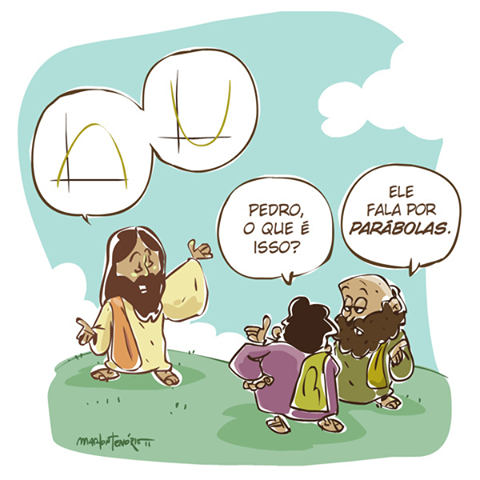
\includegraphics[scale=.5]{./imagens/25.png}
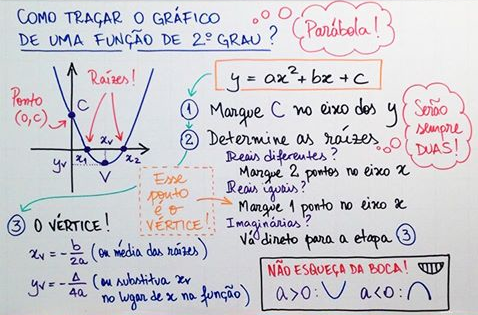
\includegraphics[scale=1]{./imagens/30.png}
\end{center}


